% Provenance (never printed): cycle 2 "Explorer les organisations du monde ---
% identifier des paysages" (littoraux, massifs montagneux, campagnes, villes),
% see sources/book1/PROVENANCE.md. Book 1, grade 1, chapter 2.
\chapter{Les paysages autour de nous}\label{ch:g1:landscapes-around-us}

Mia et son grand-père ont grimpé tout en haut de la \omterm{def:g1:landscapes-around-us:landform}{colline}, derrière le
village. Au sommet, ils s'assoient dans l'herbe pour reprendre leur
souffle, et ils regardent. En bas, les toits rouges du village se serrent
autour de l'église. Une \omterm{def:g1:landscapes-around-us:water}{rivière} serpente entre des champs verts et jaunes
et passe sous un pont. Une forêt sombre couvre la \omterm{def:g1:landscapes-around-us:landform}{colline} voisine. Et loin,
très loin, tout au bout des terres, il y a une fine ligne bleue.

«~C'est la mer~», dit son grand-père.

Tout ce que Mia peut voir du haut de la \omterm{def:g1:landscapes-around-us:landform}{colline}, de près comme de loin,
c'est un \omterm{def:g1:landscapes-around-us:landscape}{paysage}.

\begin{omfigure}
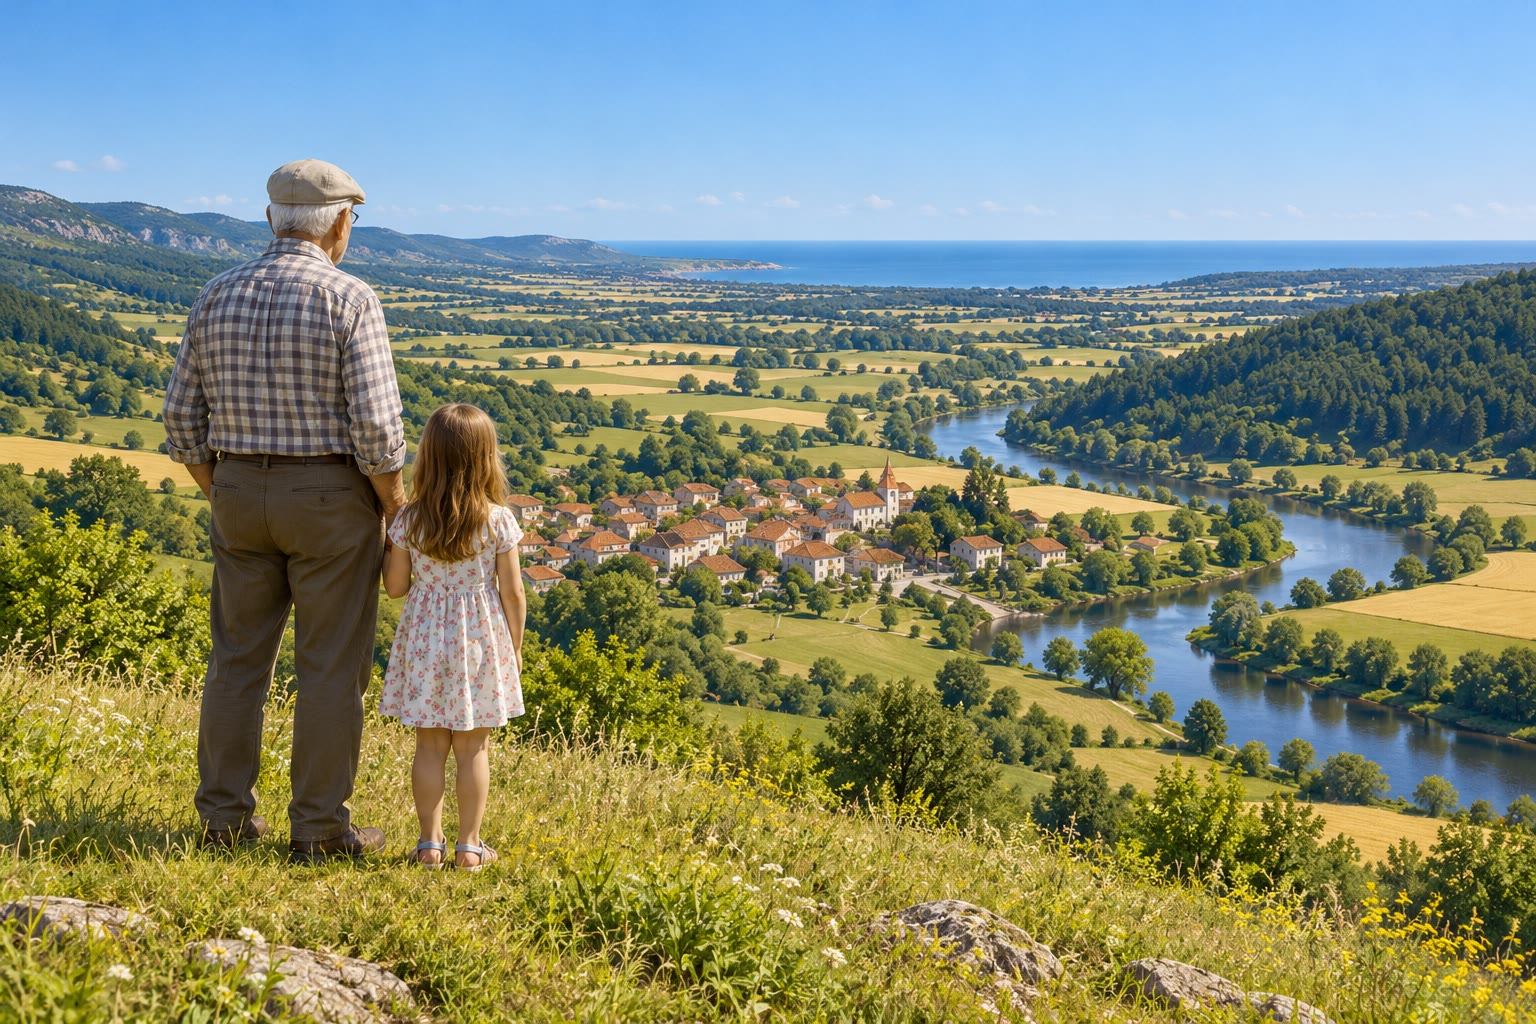
\includegraphics[width=0.72\linewidth]{images/book1/ai/g1-hilltop-view.jpg}

{\small Du haut d'une \omterm{def:g1:landscapes-around-us:landform}{colline}, on voit tout un \omterm{def:g1:landscapes-around-us:landscape}{paysage}.}
\end{omfigure}

\section{Qu'est-ce qu'un paysage~?}

\begin{definition}[Paysage]\label{def:g1:landscapes-around-us:landscape}
Un \emph{paysage}\index{paysage} est tout ce que nous voyons d'un pays d'un
seul regard, depuis l'endroit où nous sommes jusqu'à l'horizon lointain~:
la forme du sol, l'eau, les plantes, et ce que les gens ont construit.
\end{definition}

Un \omterm{def:g1:landscapes-around-us:landscape}{paysage} a des parties proches et des parties lointaines. La partie la
plus proche de nous est en bas de ce que nous voyons~; elle paraît grande
et nous en voyons les détails. La partie lointaine est en haut, près du
ciel~; elle paraît petite et pâle.

\begin{omfigure}
\begin{tikzpicture}[x=1cm, y=1cm]
  \fill[ocBlue!12] (0,0) rectangle (10,5);
  % background: far hills
  \fill[black!18] (0,3.0) -- (1.5,3.6) -- (3,3.3) -- (5,3.9) -- (7,3.4) -- (8.5,3.8) -- (10,3.3) -- (10,2.9) -- (0,2.9) -- cycle;
  % middle: hills and fields
  \fill[green!35!omLithAlluv] (0,1.6) -- (2,2.4) -- (4,2.1) -- (6,2.7) -- (8,2.2) -- (10,2.5) -- (10,1.5) -- (0,1.5) -- cycle;
  \fill[green!25!omLithAlluv] (0,1.5) rectangle (10,2.95);
  \fill[green!35!omLithAlluv] (0,2.95) -- (2,3.1) -- (4,2.95) -- (6,3.25) -- (8,3.0) -- (10,3.1) -- (10,2.9) -- (0,2.9) -- cycle;
  \foreach \x in {5.6,5.9,6.2} \fill[red!55] (\x,2.25) -- ++(0.12,0.15) -- ++(0.12,-0.15) -- cycle;
  \foreach \x in {5.6,5.9,6.2} \fill[white] (\x+0.03,2.1) rectangle ++(0.18,0.15);
  % foreground
  \fill[green!55!black!60] (0,0) rectangle (10,1.5);
  \foreach \x in {0.8,2.1,8.6} {
    \fill[brown!70!black] (\x-0.06,0.4) rectangle (\x+0.06,0.9);
    \fill[green!45!black] (\x,1.15) circle (0.38);
  }
  % band borders and labels
  \draw[white, line width=1pt, dashed] (0,1.5) -- (10,1.5);
  \draw[white, line width=1pt, dashed] (0,2.95) -- (10,2.95);
  \node[font=\small\bfseries, fill=white, fill opacity=0.8, text opacity=1, inner sep=2pt] at (5,0.6) {premier plan~: proche, grand, plein de détails};
  \node[font=\small\bfseries, fill=white, fill opacity=0.8, text opacity=1, inner sep=2pt] at (2.7,2.2) {second plan};
  \node[font=\small\bfseries, fill=white, fill opacity=0.8, text opacity=1, inner sep=2pt] at (5,4.4) {arrière-plan~: lointain, petit, pâle};
\end{tikzpicture}

{\small Un \omterm{def:g1:landscapes-around-us:landscape}{paysage} vu en trois bandes~: le premier plan en bas, le second
plan, et l'arrière-plan contre le ciel.}
\label{fig:g1:landscapes-around-us:bands}
\end{omfigure}

\section{Les formes du relief}

Le sol n'est pas plat partout. À certains endroits, il monte très haut vers
le ciel~; à d'autres, il descend dans de longs creux~; ailleurs, il est plat
à perte de vue. Nous donnons un nom à chaque forme.

\begin{definition}[Formes de relief]\label{def:g1:landscapes-around-us:landform}
Une \emph{forme de relief}\index{forme de relief} est une forme de la
surface du sol.
\begin{itemize}
  \item Une \emph{montagne}\index{montagne} est une forme de relief très
        haute, aux pentes raides~; son point le plus haut s'appelle le
        sommet. Les plus hautes montagnes gardent de la neige en haut,
        même en été.
  \item Une \emph{colline}\index{colline} est une forme de relief qui
        s'élève au-dessus du pays qui l'entoure, moins haute et plus ronde
        qu'une montagne.
  \item Une \emph{vallée}\index{vallee@vallée} est un long creux, bas,
        entre des collines ou des montagnes~; il y a souvent une \omterm{def:g1:landscapes-around-us:water}{rivière} au
        fond.
  \item Une \emph{plaine}\index{plaine} est une grande étendue de terre
        plate et basse.
\end{itemize}
\end{definition}

\begin{omfigure}
\begin{tikzpicture}[x=1cm, y=1cm]
  \fill[ocBlue!10] (0,0) rectangle (12.4,4.6);
  % sea
  \fill[omSea] (10.2,0) rectangle (12.4,0.55);
  % land profile: mountains, valley, hill, plain, coast
  \fill[omLithAlluv!80!green] (0,0) -- (0,2.2) -- (0.9,3.3) -- (1.5,3.0) -- (2.2,4.1)
     -- (2.9,2.6) -- (3.6,1.2) -- (3.9,0.9) -- (4.2,1.2) -- (5.0,2.0) -- (5.7,2.2)
     -- (6.4,1.6) -- (7.0,0.95) -- (8.0,0.8) -- (9.5,0.7) -- (10.2,0.6) -- (10.4,0.55)
     -- (10.4,0) -- cycle;
  \draw[black!60, line width=0.6pt] (0,2.2) -- (0.9,3.3) -- (1.5,3.0) -- (2.2,4.1)
     -- (2.9,2.6) -- (3.6,1.2) -- (3.9,0.9) -- (4.2,1.2) -- (5.0,2.0) -- (5.7,2.2)
     -- (6.4,1.6) -- (7.0,0.95) -- (8.0,0.8) -- (9.5,0.7) -- (10.2,0.6) -- (10.4,0.55);
  % snow caps
  \fill[white, draw=black!50, line width=0.3pt] (1.95,3.72) -- (2.2,4.1) -- (2.45,3.72) -- (2.3,3.78) -- (2.2,3.68) -- (2.08,3.78) -- cycle;
  \fill[white, draw=black!50, line width=0.3pt] (0.72,3.08) -- (0.9,3.3) -- (1.05,3.15) -- (0.9,3.12) -- cycle;
  % river in the valley
  \fill[omSea!90!black] (3.75,0.92) rectangle (4.05,0.98);
  % lake on the plain
  \fill[omSea] (7.6,0.82) ellipse (0.5 and 0.07);
  % village on the plain
  \foreach \x in {8.6,8.85,9.1} {
    \fill[white, draw=black!50, line width=0.3pt] (\x,0.74) rectangle ++(0.18,0.16);
    \fill[red!60] (\x-0.02,0.9) -- ++(0.11,0.12) -- ++(0.11,-0.12) -- cycle;
  }
  % labels
  \node[font=\small, above] at (2.2,4.12) {montagne};
  \node[font=\small, above] at (5.6,2.25) {colline};
  \node[font=\small] at (3.9,1.85) {vallée};
  \node[font=\small, above] at (8.2,1.5) {plaine};
  \draw[black!60, thin] (8.2,1.5) -- (8.2,0.85);
  \node[font=\small, align=center] at (11.3,1.4) {mer};
  \node[font=\scriptsize, below=2pt, fill=white, fill opacity=0.8, text opacity=1, inner sep=1pt] at (7.6,0.35) {lac};
  \draw[black!60, thin] (7.6,0.45) -- (7.6,0.78);
  \node[font=\scriptsize, below=2pt, fill=white, fill opacity=0.8, text opacity=1, inner sep=1pt] at (10.3,0.35) {côte};
  \node[font=\scriptsize, fill=white, fill opacity=0.8, text opacity=1, inner sep=1pt] at (3.9,0.2) {rivière};
  \draw[black!60, thin] (3.9,0.32) -- (3.9,0.88);
\end{tikzpicture}

{\small Les formes du relief, des \omterm{def:g1:landscapes-around-us:landform}{montagnes} jusqu'à la mer, vues de côté
(les hauteurs sont dessinées bien plus grandes qu'en vrai).}
\label{fig:g1:landscapes-around-us:profile}
\end{omfigure}

\begin{omfigure}
\begin{minipage}[b]{0.49\linewidth}\centering
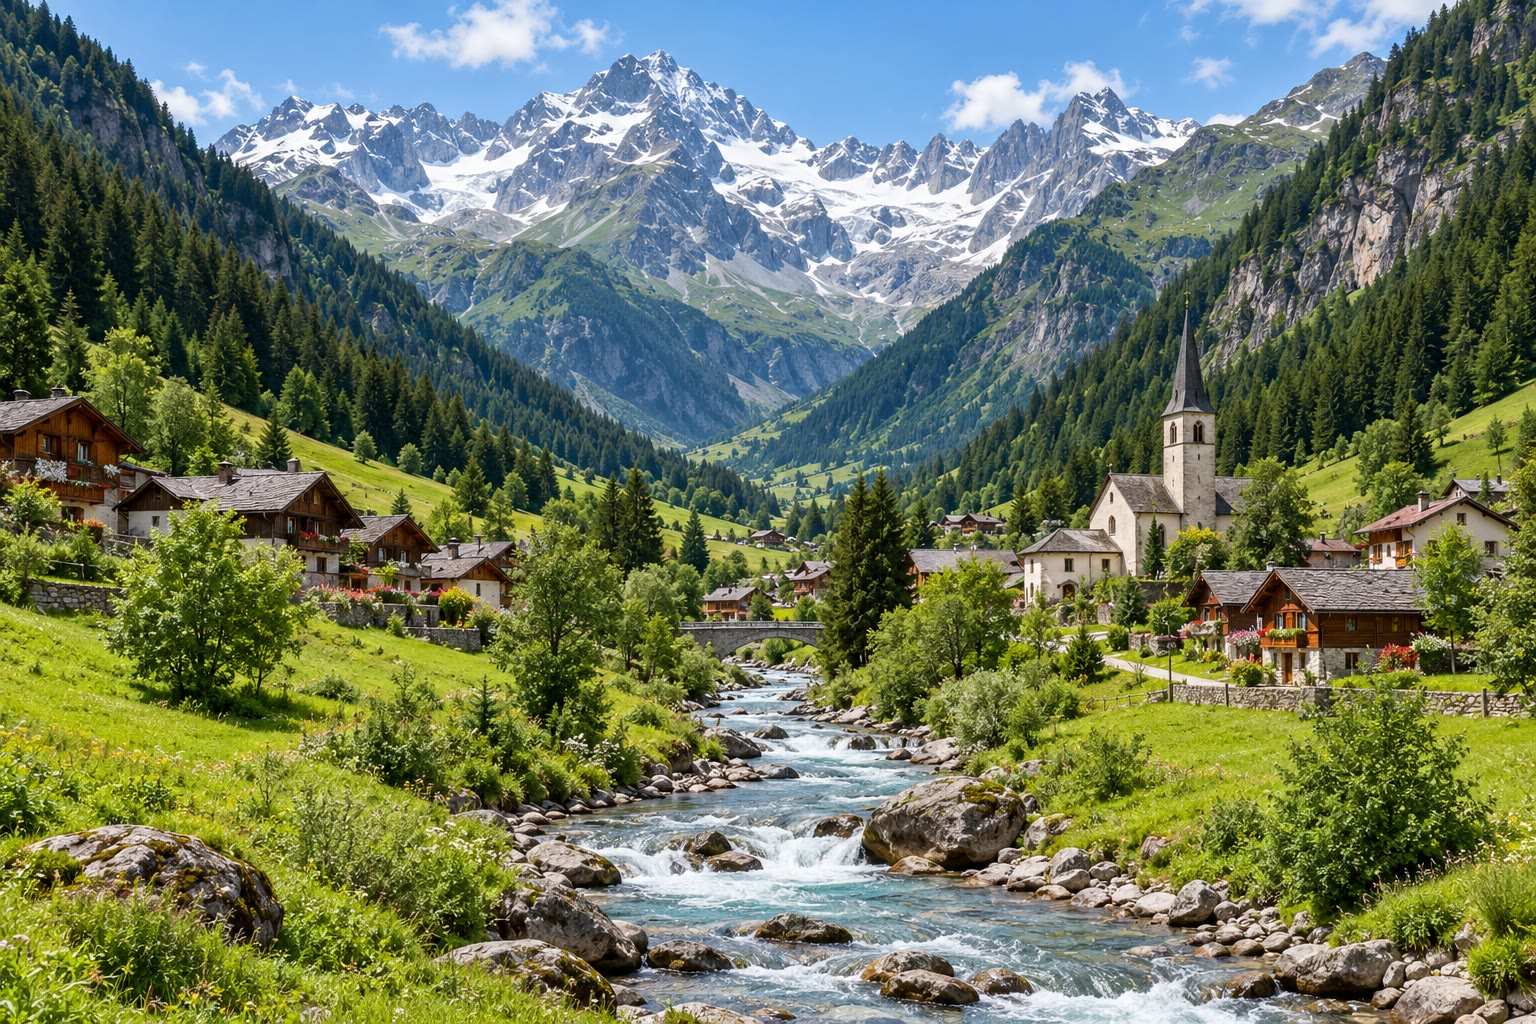
\includegraphics[width=\linewidth]{images/book1/ai/g1-mountain-village.jpg}

{\small Des \omterm{def:g1:landscapes-around-us:landform}{montagnes}, et un village dans leur \omterm{def:g1:landscapes-around-us:landform}{vallée}.}
\end{minipage}\hfill
\begin{minipage}[b]{0.49\linewidth}\centering
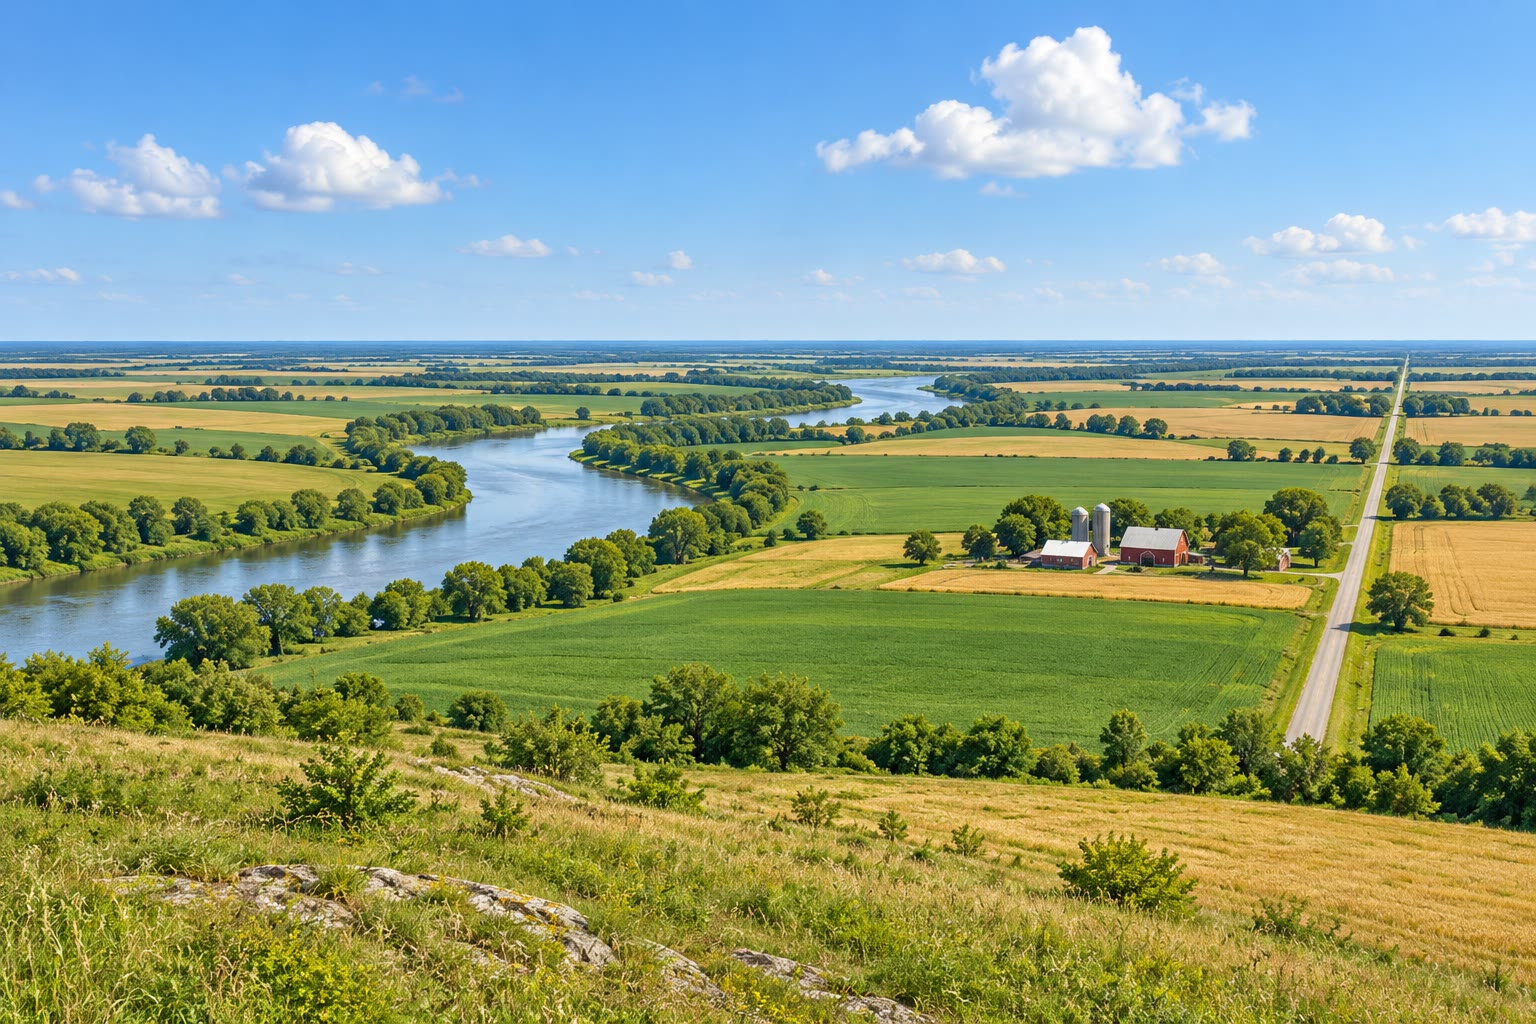
\includegraphics[width=\linewidth]{images/book1/ai/g1-plain-river.jpg}

{\small Une \omterm{def:g1:landscapes-around-us:landform}{plaine}, avec une \omterm{def:g1:landscapes-around-us:water}{rivière} et des champs.}
\end{minipage}
\end{omfigure}

\begin{example}[Montagne ou colline~?]\label{ex:g1:landscapes-around-us:mountain-hill}
Il n'existe pas de hauteur exacte à partir de laquelle une \omterm{def:g1:landscapes-around-us:landform}{colline} devient
une \omterm{def:g1:landscapes-around-us:landform}{montagne}. Nous regardons la forme~: une \omterm{def:g1:landscapes-around-us:landform}{montagne} est haute et raide,
souvent rocheuse, parfois couverte de neige au sommet~; une \omterm{def:g1:landscapes-around-us:landform}{colline} est
plus basse et plus ronde, souvent couverte d'herbe, de champs ou de bois,
et on peut monter à son sommet en peu de temps.
\end{example}

\section{L'eau dans le paysage}

L'eau fait partie de la plupart des \omterm{def:g1:landscapes-around-us:landscape}{paysages}. Elle descend des \omterm{def:g1:landscapes-around-us:landform}{collines} et
des \omterm{def:g1:landscapes-around-us:landform}{montagnes}, se rassemble dans les creux et rejoint la mer.

\begin{definition}[L'eau dans un paysage]\label{def:g1:landscapes-around-us:water}
Une \emph{rivière}\index{riviere@rivière} est de l'eau qui coule tout le
temps dans un long chenal, des terres hautes jusqu'à un lac ou jusqu'à la
mer. Un \emph{lac}\index{lac} est une grande étendue d'eau entourée de
terre. La \emph{côte}\index{cote@côte} est l'endroit où la terre rencontre
la mer.
\end{definition}

\begin{omfigure}
\begin{minipage}[b]{0.49\linewidth}\centering
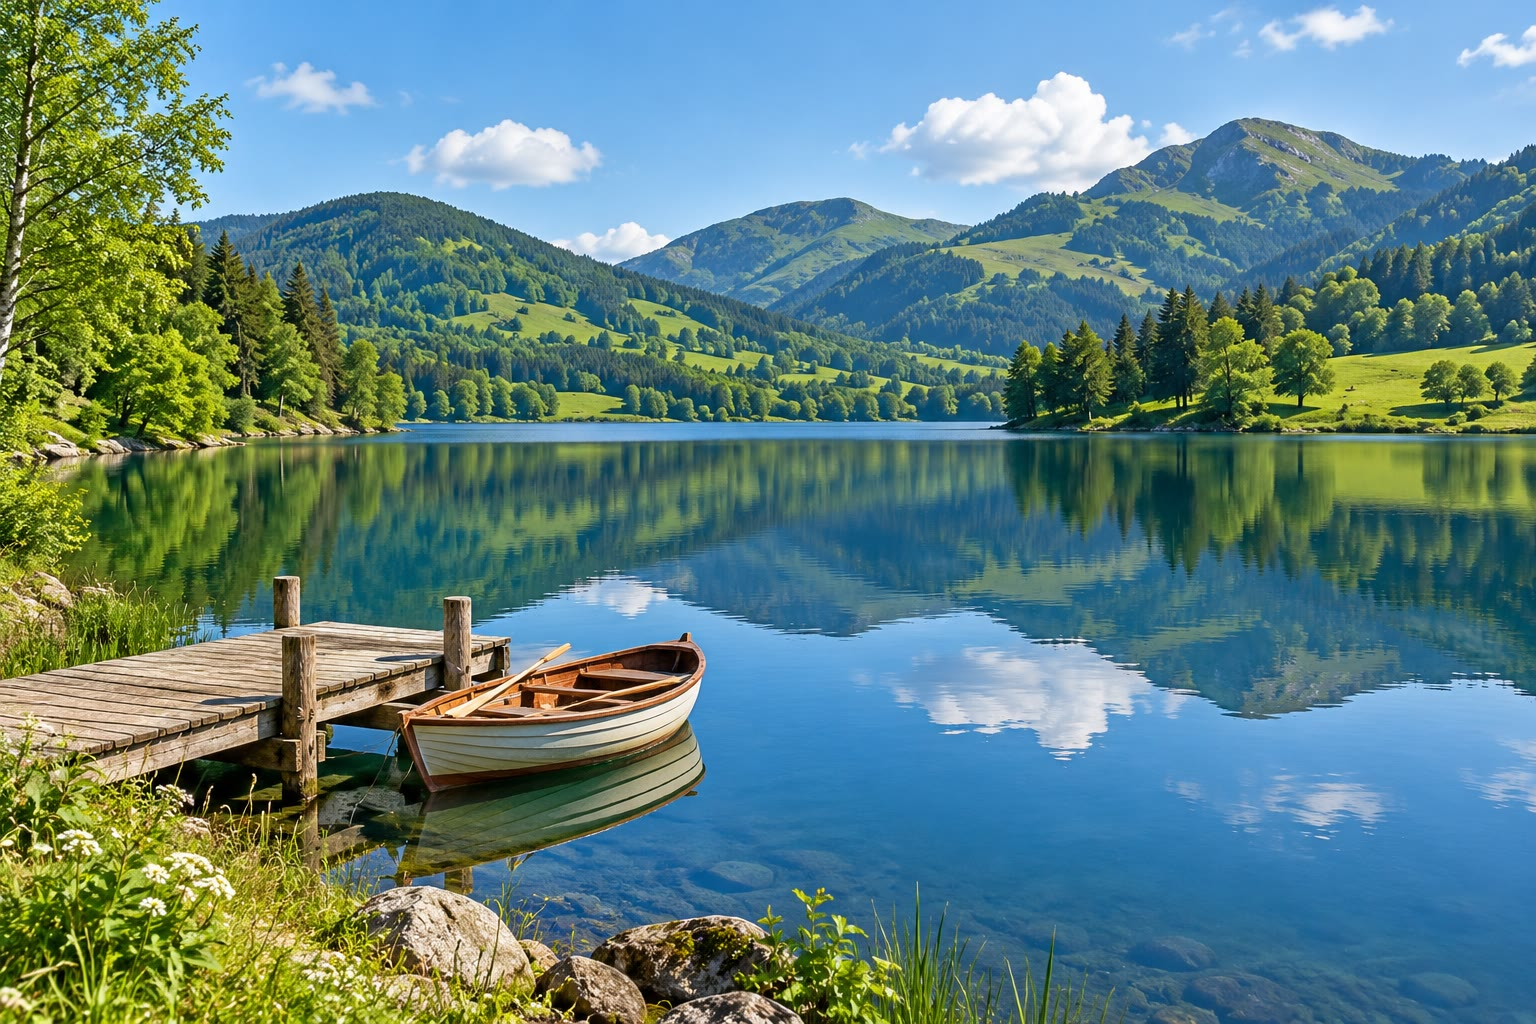
\includegraphics[width=\linewidth]{images/book1/ai/g1-lake-hills.jpg}

{\small Un \omterm{def:g1:landscapes-around-us:water}{lac} au milieu des \omterm{def:g1:landscapes-around-us:landform}{collines}.}
\end{minipage}\hfill
\begin{minipage}[b]{0.49\linewidth}\centering
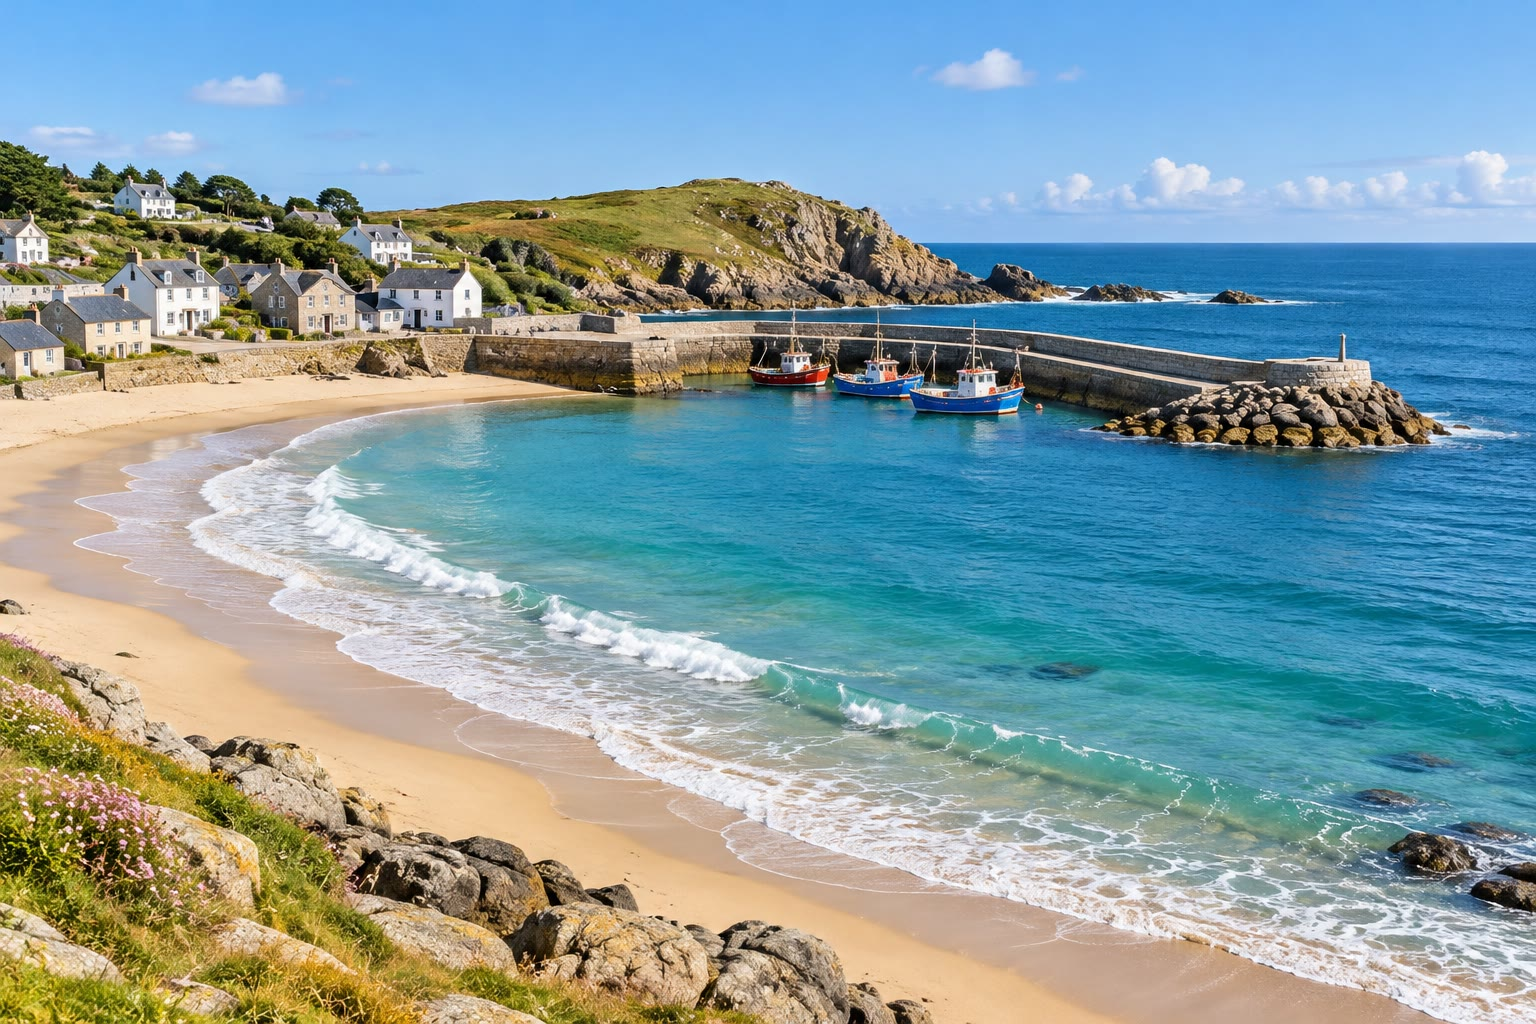
\includegraphics[width=\linewidth]{images/book1/ai/g1-coast-harbour.jpg}

{\small Une \omterm{def:g1:landscapes-around-us:water}{côte}~: une plage, des rochers et un port.}
\end{minipage}
\end{omfigure}

\begin{remark}[L'eau descend toujours la pente]\label{rem:g1:landscapes-around-us:downhill}
Une \omterm{def:g1:landscapes-around-us:water}{rivière} coule toujours d'un endroit plus haut vers un endroit plus bas.
C'est pour cela que les \omterm{def:g1:landscapes-around-us:water}{rivières} coulent au fond des \omterm{def:g1:landscapes-around-us:landform}{vallées}, et qu'elles
finissent par rejoindre un \omterm{def:g1:landscapes-around-us:water}{lac} ou la mer, qui sont plus bas que les terres
autour d'eux.
\end{remark}

\section{Les éléments naturels et les éléments construits}

Certaines parties d'un \omterm{def:g1:landscapes-around-us:landscape}{paysage} étaient là avant l'arrivée des gens~: les
\omterm{def:g1:landscapes-around-us:landform}{montagnes}, les \omterm{def:g1:landscapes-around-us:water}{rivières}, les forêts. D'autres parties ont été faites par
les gens~: les maisons, les routes, les ponts, les champs.

\begin{definition}[Éléments naturels et éléments construits]\label{def:g1:landscapes-around-us:natural-built}
Un \emph{élément naturel}\index{element naturel@élément naturel} d'un
\omterm{def:g1:landscapes-around-us:landscape}{paysage} est une partie qui n'a pas été faite par les gens~: une \omterm{def:g1:landscapes-around-us:landform}{montagne},
une \omterm{def:g1:landscapes-around-us:water}{rivière}, un \omterm{def:g1:landscapes-around-us:water}{lac}, une forêt, une plage. Un
\emph{élément construit}\index{element construit@élément construit} est une
partie faite ou façonnée par les gens~: une maison, une route, un pont, un
port, un champ, un jardin.
\end{definition}

\begin{omfigure}
\begin{tikzpicture}[x=1cm, y=1cm]
  \node[draw=omDef!80!black, fill=omDef!10, rounded corners, text width=5.2cm,
        align=left, minimum height=3.2cm, anchor=north] (n) at (0,0)
    {\textbf{naturel}\\[2pt] montagne\\ colline\\ vallée\\ rivière\\ lac\\ forêt\\ plage};
  \node[draw=omMeth!80!black, fill=omMeth!10, rounded corners, text width=5.2cm,
        align=left, minimum height=3.2cm, anchor=north] (b) at (6,0)
    {\textbf{construit par les gens}\\[2pt] maison\\ église\\ route\\ pont\\ port\\ champ\\ jardin};
\end{tikzpicture}

{\small On trie les éléments du \omterm{def:g1:landscapes-around-us:landscape}{paysage} de Mia. Un champ est construit~:
les gens ont défriché la terre et l'ont cultivée.}
\label{fig:g1:landscapes-around-us:sort}
\end{omfigure}

\section{Les paysages changent}

Un \omterm{def:g1:landscapes-around-us:landscape}{paysage} ne reste pas le même pour toujours. Certains changements sont
rapides, et d'autres si lents que personne ne les voit au cours d'une vie.
\begin{itemize}
  \item \textbf{Avec les saisons~:} les champs sont bruns après le
        labour, verts au printemps, dorés avant la moisson~; les arbres
        perdent leurs feuilles en automne~; la neige peut tout recouvrir en
        hiver.
  \item \textbf{À cause des gens~:} un village grandit et devient une
        ville~; une forêt est coupée pour faire des champs~; une nouvelle
        route et un pont traversent la \omterm{def:g1:landscapes-around-us:landform}{vallée}.
  \item \textbf{À cause de l'eau et du \omterm{def:g1:watching-the-weather:weather}{temps qu'il fait}~:} après un gros
        orage, une \omterm{def:g1:landscapes-around-us:water}{rivière} peut sortir de son lit et couvrir les champs
        pendant quelques jours~; sur la \omterm{def:g1:landscapes-around-us:water}{côte}, les vagues usent lentement
        les rochers.
\end{itemize}

\begin{omfigure}
\begin{tikzpicture}[x=1cm, y=1cm]
  \foreach \k/\t in {0/autrefois, 1/aujourd'hui} {
  \begin{scope}[shift={(\k*6.4,0)}]
    \fill[ocBlue!8] (0,0) rectangle (5.8,3.4);
    \fill[green!30!omLithAlluv] (0,0) rectangle (5.8,1.9);
    % river
    \fill[omSea] (0,0.55) .. controls (1.5,0.9) and (2.5,0.2) .. (5.8,0.6)
       -- (5.8,0.85) .. controls (2.5,0.45) and (1.5,1.15) .. (0,0.8) -- cycle;
    % hill
    \fill[green!45!black!55] (2.8,1.9) .. controls (3.8,3.1) and (4.8,3.1) .. (5.8,2.2) -- (5.8,1.9) -- cycle;
    \ifnum\k=0
      % forest everywhere, a few houses
      \foreach \x in {0.4,0.9,1.4,1.9,2.4,4.3,4.8,5.3}
        \fill[green!40!black] (\x,1.45) circle (0.22);
      \foreach \x in {3.4,3.75} {
        \fill[white, draw=black!50, line width=0.3pt] (\x,1.15) rectangle ++(0.24,0.2);
        \fill[red!60] (\x-0.03,1.35) -- ++(0.15,0.14) -- ++(0.15,-0.14) -- cycle; }
    \else
      % fields, many houses, a road and a bridge
      \foreach \x/\c in {0.1/yellow!60, 1.3/green!55, 4.5/yellow!45}
        \fill[\c] (\x,1.05) rectangle ++(1.1,0.5);
      \fill[black!35] (2.65,0) rectangle (2.95,1.9);
      \fill[black!55] (2.55,0.5) rectangle (3.05,0.9);
      \foreach \x in {3.2,3.55,3.9} \foreach \y in {1.1,1.45} {
        \fill[white, draw=black!50, line width=0.3pt] (\x,\y) rectangle ++(0.24,0.2);
        \fill[red!60] (\x-0.03,\y+0.2) -- ++(0.15,0.14) -- ++(0.15,-0.14) -- cycle; }
      \foreach \x in {4.6,5.2} \fill[green!40!black] (\x,2.35) circle (0.2);
    \fi
    \node[font=\small\bfseries] at (2.9,-0.3) {\t};
  \end{scope}}
\end{tikzpicture}

{\small La même \omterm{def:g1:landscapes-around-us:landform}{vallée} autrefois et aujourd'hui. La \omterm{def:g1:landscapes-around-us:landform}{colline} et la \omterm{def:g1:landscapes-around-us:water}{rivière}
n'ont pas bougé~; les gens ont coupé presque toute la forêt, fait des
champs, construit d'autres maisons, une route et un pont.}
\label{fig:g1:landscapes-around-us:change}
\end{omfigure}

\begin{example}[La ville et la campagne]\label{ex:g1:landscapes-around-us:town}
En ville, presque tout ce que nous voyons a été construit~: les rues, les
maisons, les magasins, les ponts, les parcs. À la campagne, nous voyons
surtout des champs, des bois et des prés, avec quelques fermes et quelques
villages. Les deux sont des \omterm{def:g1:landscapes-around-us:landscape}{paysages}. Même au milieu d'une grande ville,
les formes du relief sont toujours là~: une \omterm{def:g1:landscapes-around-us:water}{rivière} traverse la ville, et
certaines rues montent sur une \omterm{def:g1:landscapes-around-us:landform}{colline}.
\end{example}

\section{Décrire un paysage}

\begin{method}[Décrire un paysage en quatre étapes]\label{met:g1:landscapes-around-us:describe}
Pour décrire un \omterm{def:g1:landscapes-around-us:landscape}{paysage}, du haut d'une \omterm{def:g1:landscapes-around-us:landform}{colline} ou sur une image~:
\begin{enumerate}
  \item \textbf{Partage-le en trois bandes~:} le premier plan, le second
        plan et l'arrière-plan.
  \item \textbf{Nomme les formes du relief~:} \omterm{def:g1:landscapes-around-us:landform}{montagnes}, \omterm{def:g1:landscapes-around-us:landform}{collines}, \omterm{def:g1:landscapes-around-us:landform}{vallées},
        \omterm{def:g1:landscapes-around-us:landform}{plaines}.
  \item \textbf{Trouve l'eau~:} une \omterm{def:g1:landscapes-around-us:water}{rivière}, un \omterm{def:g1:landscapes-around-us:water}{lac}, la mer et sa \omterm{def:g1:landscapes-around-us:water}{côte}.
  \item \textbf{Trouve ce que les gens ont construit~:} maisons, routes,
        ponts, champs.
\end{enumerate}
\end{method}

\begin{example}[Le paysage de Mia]\label{ex:g1:landscapes-around-us:mia}
Au premier plan, l'herbe du haut de la \omterm{def:g1:landscapes-around-us:landform}{colline}. Au second plan, une \omterm{def:g1:landscapes-around-us:landform}{vallée}
avec une \omterm{def:g1:landscapes-around-us:water}{rivière}, un pont et un village, des champs autour, et une forêt
sur la \omterm{def:g1:landscapes-around-us:landform}{colline} voisine. À l'arrière-plan, une \omterm{def:g1:landscapes-around-us:landform}{plaine} et, au bout des
terres, la \omterm{def:g1:landscapes-around-us:water}{côte} et la mer. Naturels~: les \omterm{def:g1:landscapes-around-us:landform}{collines}, la \omterm{def:g1:landscapes-around-us:landform}{vallée}, la \omterm{def:g1:landscapes-around-us:water}{rivière},
la forêt, la mer. Construits~: le village, l'église, le pont, les champs.
\end{example}

\section{Exercices}

\begin{exercise}[$\star$]\label{exo:g1:landscapes-around-us:1}
Nomme les quatre \omterm{def:g1:landscapes-around-us:landform}{formes de relief} que tu as apprises dans ce chapitre.
\end{exercise}

\begin{exercise}[$\star$]\label{exo:g1:landscapes-around-us:2}
Laquelle est la plus haute et la plus raide~: une \omterm{def:g1:landscapes-around-us:landform}{colline} ou une \omterm{def:g1:landscapes-around-us:landform}{montagne}~?
\end{exercise}

\begin{exercise}[$\star$]\label{exo:g1:landscapes-around-us:3}
Naturel ou construit~? Une \omterm{def:g1:landscapes-around-us:water}{rivière}~; une route~; une forêt~; un pont~; une plage~; une maison.
\end{exercise}

\begin{exercise}[$\star$]\label{exo:g1:landscapes-around-us:4}
Où est la \omterm{def:g1:landscapes-around-us:water}{côte}~: là où la terre rencontre une \omterm{def:g1:landscapes-around-us:water}{rivière}, ou là où la terre
rencontre la mer~?
\end{exercise}

\begin{exercise}[$\star$]\label{exo:g1:landscapes-around-us:5}
Regarde l'image des \omterm{def:g1:landscapes-around-us:landform}{montagnes} et de leur village. Nomme un \omterm{def:g1:landscapes-around-us:natural-built}{élément naturel}
et un \omterm{def:g1:landscapes-around-us:natural-built}{élément construit}.
\end{exercise}

\begin{exercise}[$\star$]\label{exo:g1:landscapes-around-us:6}
Sur le dessin des formes du relief, quelle \omterm{def:g1:landscapes-around-us:landform}{forme de relief} est la plus
haute~? Où coule la \omterm{def:g1:landscapes-around-us:water}{rivière}~?
\end{exercise}

\begin{exercise}[$\star\star$]\label{exo:g1:landscapes-around-us:7}
D'où vient une \omterm{def:g1:landscapes-around-us:water}{rivière}, et où va-t-elle~? Pourquoi ne monte-t-elle jamais
jusqu'en haut d'une \omterm{def:g1:landscapes-around-us:landform}{colline}~?
\end{exercise}

\begin{exercise}[$\star\star$]\label{exo:g1:landscapes-around-us:8}
Sur l'image d'un \omterm{def:g1:landscapes-around-us:landscape}{paysage}, un arbre en bas de l'image paraît plus grand
qu'une \omterm{def:g1:landscapes-around-us:landform}{colline} entière en haut. Pourquoi~?
\end{exercise}

\begin{exercise}[$\star\star$]\label{exo:g1:landscapes-around-us:9}
Décris l'image de la \omterm{def:g1:landscapes-around-us:landform}{plaine} et de sa \omterm{def:g1:landscapes-around-us:water}{rivière} en trois bandes~: qu'y a-t-il
au premier plan, au second plan et à l'arrière-plan~?
\end{exercise}

\begin{exercise}[$\star\star$]\label{exo:g1:landscapes-around-us:10}
Un champ de blé est vert ou doré, comme l'herbe. Pourquoi dit-on que c'est
un \omterm{def:g1:landscapes-around-us:natural-built}{élément construit} du \omterm{def:g1:landscapes-around-us:landscape}{paysage}, et non un \omterm{def:g1:landscapes-around-us:natural-built}{élément naturel}~?
\end{exercise}

\begin{exercise}[$\star\star$]\label{exo:g1:landscapes-around-us:11}
Regarde le dessin de la \omterm{def:g1:landscapes-around-us:landform}{vallée} autrefois et aujourd'hui. Nomme deux choses
qui n'ont pas changé et trois choses que les gens ont ajoutées.
\end{exercise}
